\chapter{Visualisations of Topological Charge Distributions}
\label{app:vis}

    \graphicspath{{Appendices_Folder/figures/PNG/}{Appendices_Folder/figures/PDF/}{Appendices_Folder/figures/}}

A number of visualisations were carried out on the topological charge distribution of a single $64\times{32}^3$ lattice configuration of \lmwt at $\beta=2.05,m=-1.51$, using the VisIt visualisation tool \cite{Childs:2005:ACS,visit-website}. Positive and negative topological charge are shown in orange and blue respectively.

In figure \ref{fig:timeslices} a single timeslice is shown both before cooling and after 20 cools. Both cases are normalised by the maxima in the distribution; in spite of this, the gauge noise is clearly dominating in the uncooled case. In the cooled case, the individual instantons can be seen easily. Figure \ref{fig:timeslice-ring} shows another timeslice, this time showing each cooling step in addition to the uncooled case. Figure \marginnote{corrected cross-reference}\ref{fig:tall-ring} adds in the time dimension: each cube is still a 3-dimensional time slice, and the time dimension runs around the ring. Moving down the columns gives the successively cooled versions of the same time slice, up to 20 cools. The removal of the noise is still clearly visible, and the plateau mentioned in chapter \ref{ch:topology} between 10 and 20 cools that allows relative flexibility in the choice of cooling can be observed in the lower half of the image. This image was submitted to Swansea University's Research as Art and the Royal Society's Picturing Science events, \marginnote{added comment}and was selected as the winner of the Postgraduate Award at the former.

\begin{figure}
\centering

\begin{subfigure}[b]{0.35\textwidth}
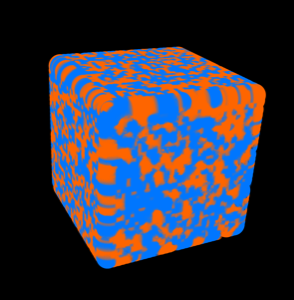
\includegraphics[width=\textwidth]{0cool.png}

\caption{Before cooling.}
\end{subfigure}
\qquad\qquad
\begin{subfigure}[b]{0.35\textwidth}
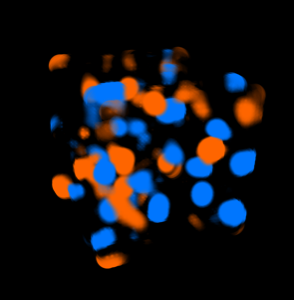
\includegraphics[width=\textwidth]{20cool.png}

\caption{After 20 cools.}
\end{subfigure}

\caption{The topological charge distribution of a single timeslice, before and after cooling. Rendering was performed using a Mac Pro machine in Swansea University as the frontend, and the BlueIce2 cluster in Swansea University as the backend, using 480 compute cores across 40 nodes. }
\label{fig:timeslices}
\end{figure}

\begin{figure}
\centering
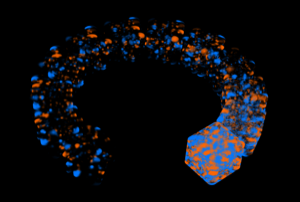
\includegraphics[width=\textwidth]{torus0010.png}

\caption{The topological charge distribution of a single timeslice. Moving anticlockwise around the ring takes us from the uncooled case to 10 cools. Rendering was performed using the Mac Pro used in figure \ref{fig:timeslices} as both front and backend. }
\label{fig:timeslice-ring}
\end{figure}

\begin{figure}
\centering
\marginnote{Lightened image to represent winning condition}
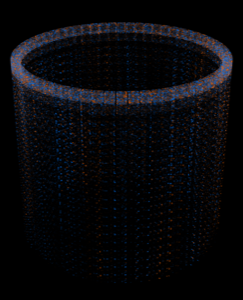
\includegraphics[width=\textwidth]{torus0032.png}

\caption{The topological charge distribution of all 64 timeslices of the configuration. Moving around the ring takes us around the time dimension, while moving down the columns takes us from the uncooled state to 20 cools. This gives a total of 1344 cubes. Rendering was performed using the machine combination used for figure \ref{fig:timeslices}.}
\label{fig:tall-ring}
\end{figure}
